\chapter{实验装置}

冷原子真空计量实验的成功实现依赖于一套复杂精密的实验平台。该平台的核心在于构建三大子系统：\textbf{超高真空系统}、\textbf{激光冷却系统}以及\textbf{磁场系统}。其中，超高真空环境旨在有效抑制背景气体碰撞，是实现长寿命原子俘获与精确真空计量的物理基础；激光系统主要负责原子的冷却、俘获与量子态制备；磁场系统则用于构建势阱以稳定囚禁原子。

本章将对上述关键子系统进行分模块的详细阐述。首先介绍真空系统的整体结构以及超高真空环境的维持和监测机制，随后讨论激光系统的光路设计，最后对磁场系统进行说明。实验装置主体外观如图\ref{fig:ch2-1}所示。

\begin{figure}[htbp]
	\centering
	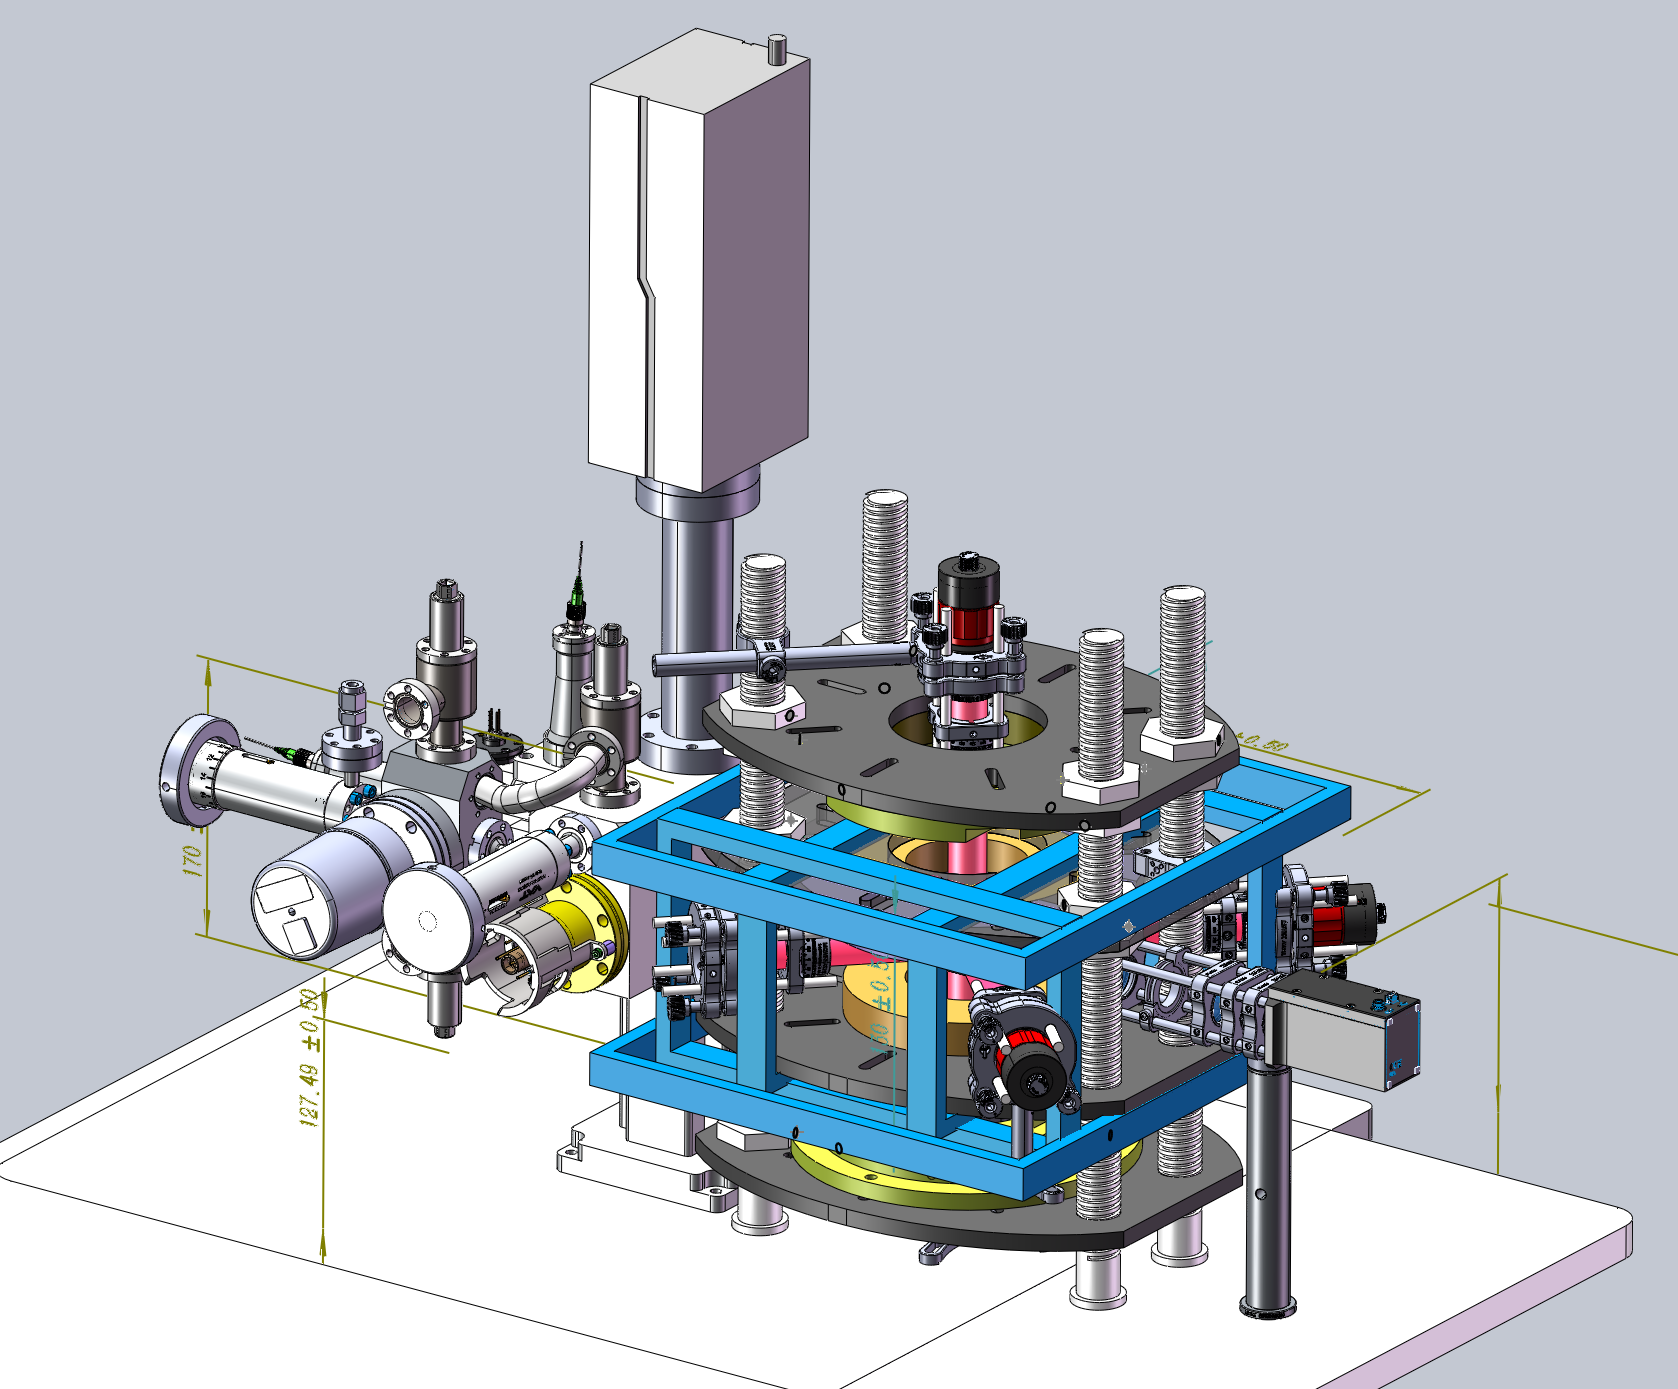
\includegraphics[width=0.6\linewidth]{figs/ch2-1.png}
	\caption{实验装置主体的三维视图}
	\label{fig:ch2-1}
\end{figure}

\section{真空系统}

实现超高真空条件下的精确计量，首要前提是构建一个长期稳定且可控的超高真空环境。本实验所采用的超高真空腔体构成了整个装置的核心平台。本节将从真空系统的机械结构、残余气体成分分析以及真空环境的维持与实时监测三个方面进行详细介绍。

\subsection{真空系统的结构}

真空腔体的整体结构如图\ref{fig:ch2-3}所示，系统由二维磁光阱（Two-dimensional Magneto-optical Trap, 2D MOT）、三维磁光阱（Three-dimensional Magneto-optical Trap, 3D MOT）、复合抽气系统以及真空计量模块等多个功能单元构成。

\begin{figure}[htbp]
	\centering
	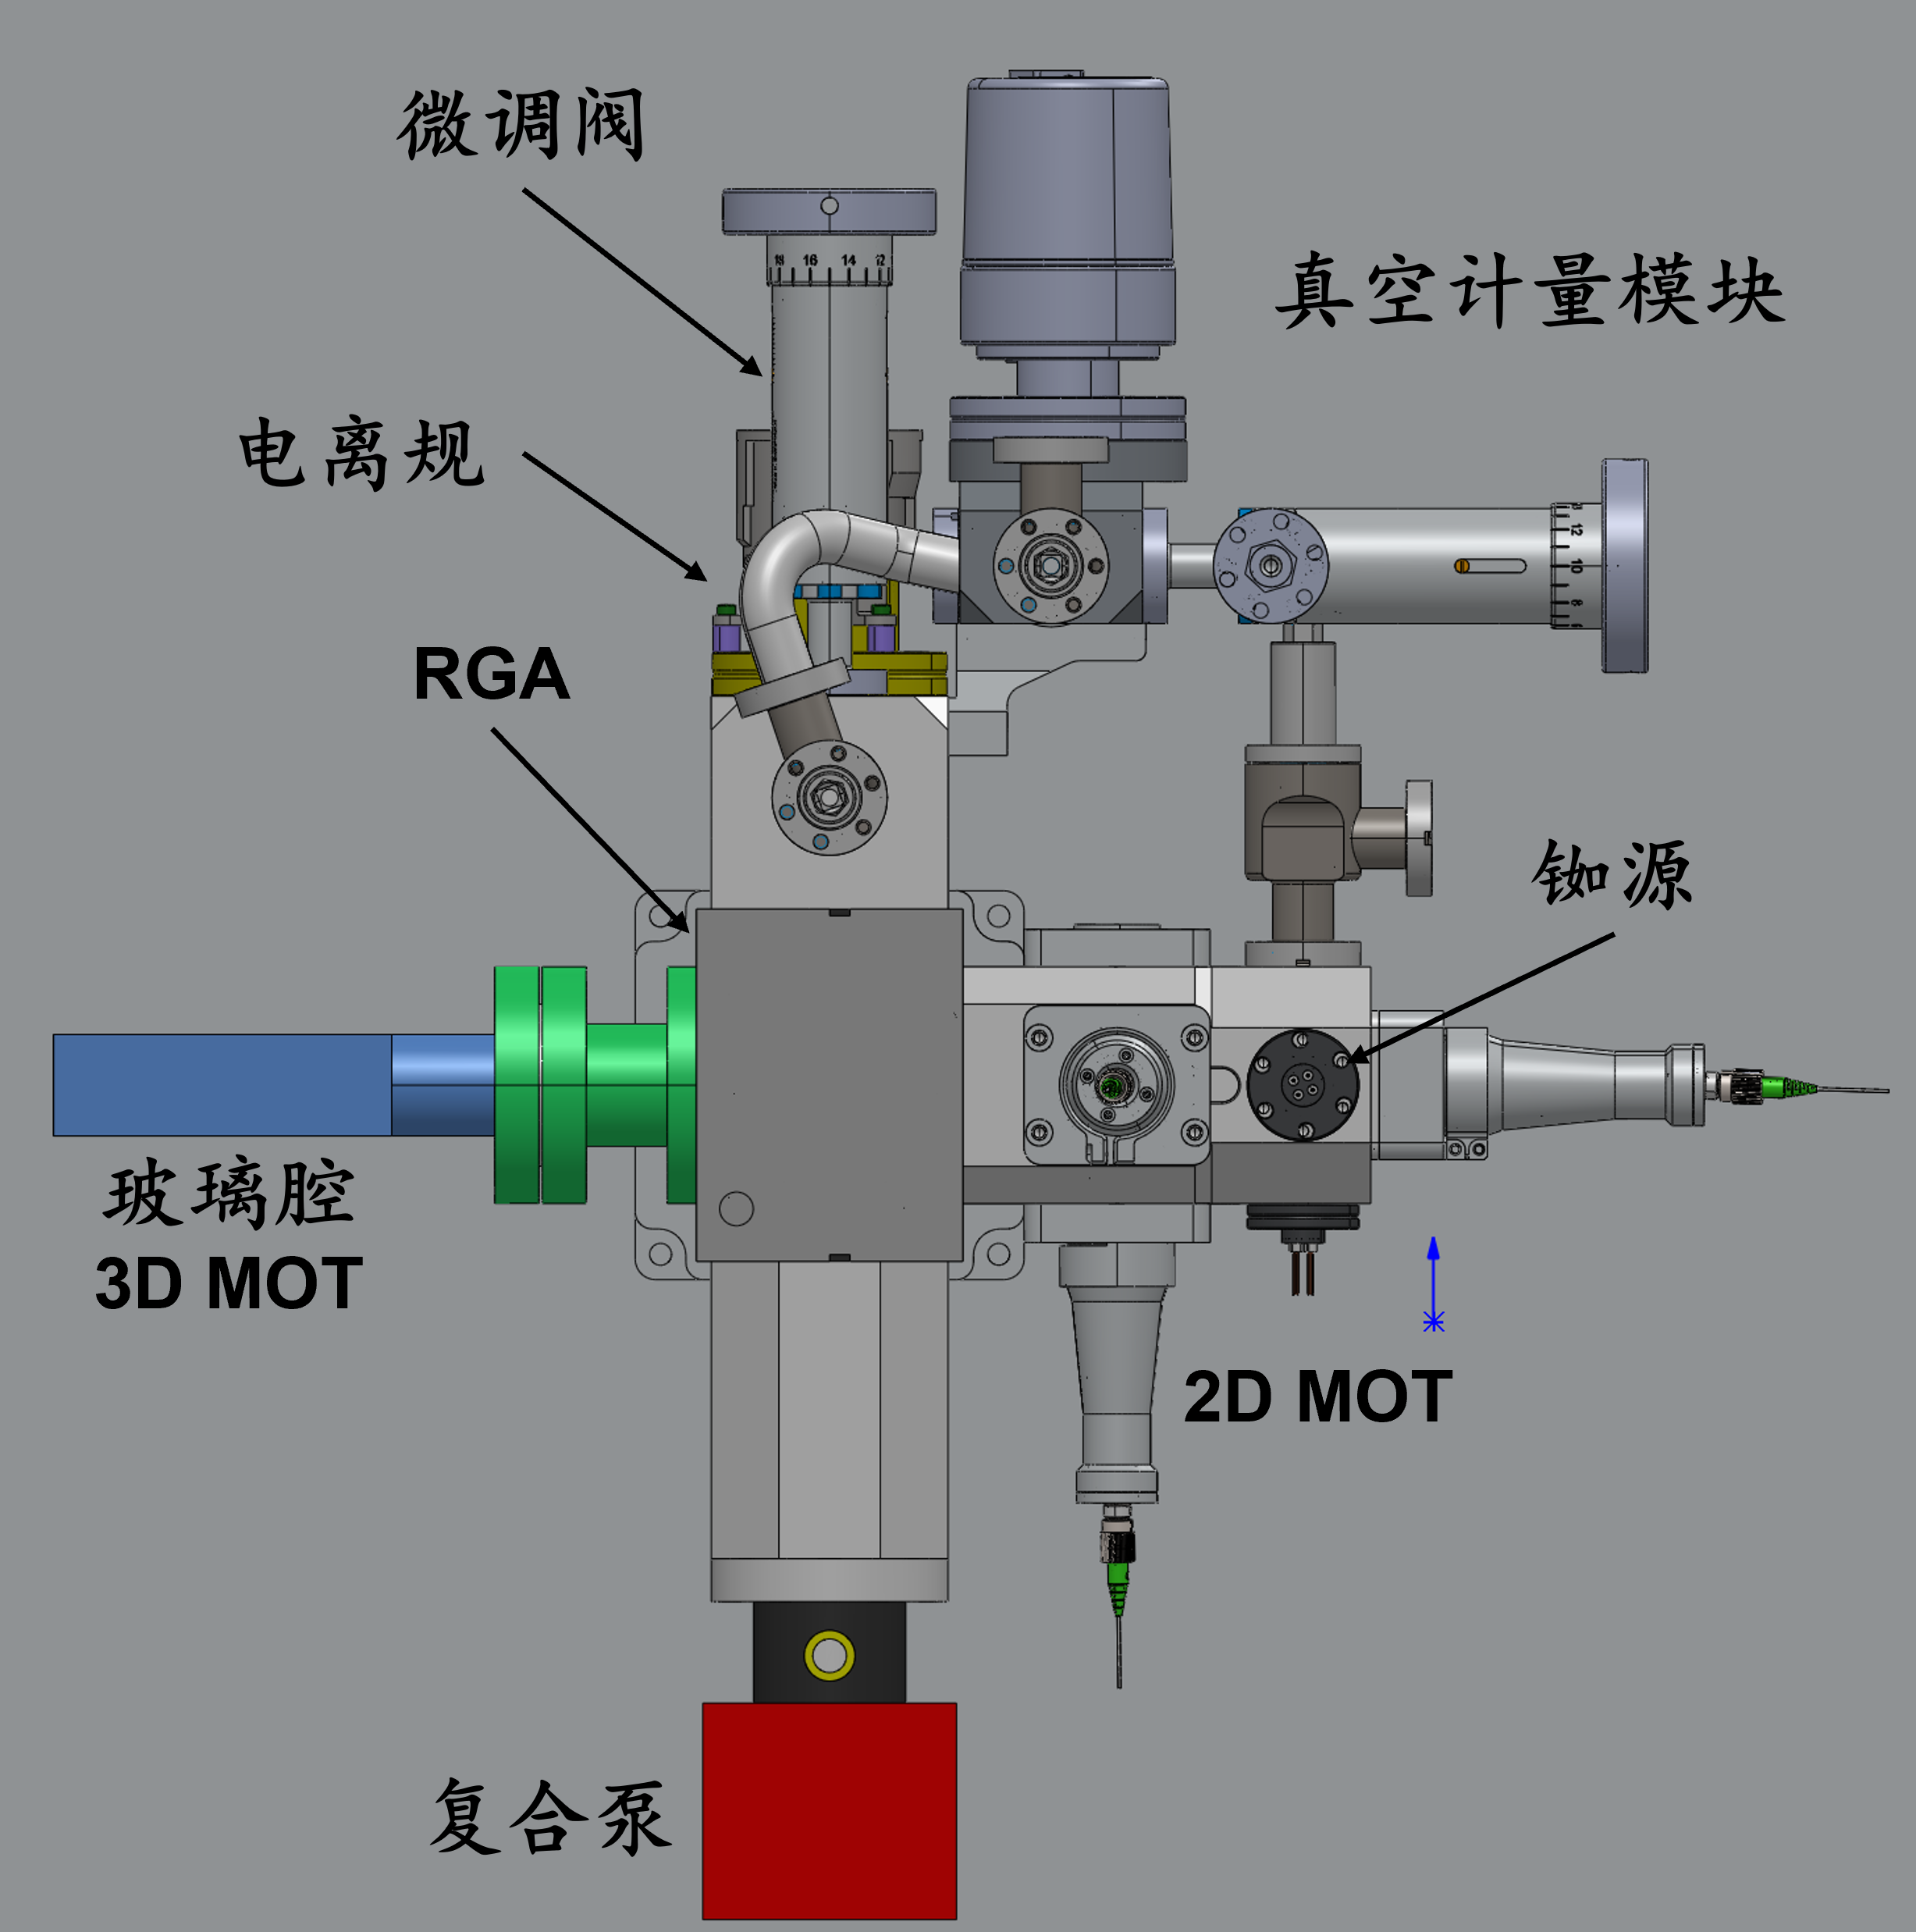
\includegraphics[width=0.6\linewidth]{figs/ch2-3.png}
	\caption{真空系统的俯视图}
	\label{fig:ch2-3}
\end{figure}

2D MOT 区域内部集成有碱金属释放器（dispenser），其内封装高纯度铷源。通过对内置电热丝通电加热，可释放铷蒸气，其中包含自然丰度分布的 $^{85}\mathrm{Rb}$ 与 $^{87}\mathrm{Rb}$ 同位素。实验中可根据需求选择性俘获特定同位素，从而实现不同工作模式的切换。此外，2D MOT 腔体配置有五个高透过率光学窗口，用于引入冷却光与推送光束；窗口外侧环绕安装有磁场线圈，以产生二维磁光阱所需的梯度磁场。

在 2D MOT 区域中，铷原子首先被预冷却并俘获，随后形成具有一定方向性的原子束流，通过差分抽气结构注入至 3D MOT 区域。3D MOT 区域采用镀膜玻璃腔体，并通过法兰与主真空系统连接。由于 2D MOT 需要维持相对较高的铷蒸气分压以提高装载效率，而 3D MOT 对背景气体碰撞极为敏感，因此实验中采用差分管实现两区域的连接与隔离，从而在保证原子通量的同时维持显著的压力梯度，使 3D MOT 区域达到超高真空水平。

为维持系统所需的超高真空环境，真空腔体配备了复合型抽气系统（通常包括离子泵与非蒸发吸气泵），用于持续清除腔体内的残余气体分子，从而保证系统的长期稳定运行。

真空计量模块主要由微调阀、波纹管等气路组件构成，用于实现高纯气体的精确引入。模块中集成高精度电离规，用于实时监测腔体压强，并为冷原子真空计量提供传统测量手段的对照基准。此外，系统顶部还安装有残余气体分析仪（Residual Gas Analyzer, RGA），如图\ref{fig:ch2-1}所示，可对腔体内气体成分及其分压进行定量分析。

\subsection{真空系统中残余气体成分分析}

在小型化冷原子真空计量系统中，不同背景气体分子与铷原子之间的碰撞截面存在显著差异，从而直接影响基于原子损失率的压强反演结果。因此，在实验开展之前，有必要对真空腔体内残余气体的组分及其分压进行定量分析，以确定适用于压强反演计算的有效碰撞截面参数。

本实验采用美国斯坦福研究系统（Stanford Research Systems, SRS）RGA100 残余气体分析仪（Residual Gas Analyzer, RGA），如图\ref{fig:ch2-6}所示。该设备可在 $1 \sim 100~\mathrm{amu}$ 的质量范围内对气体组分进行分辨，并实现各组分分压的定量测量\cite{ResidualGasAnalyzer}，为后续冷原子真空计量中的压强反演提供关键实验依据。

\begin{figure}[htbp]
	\centering
	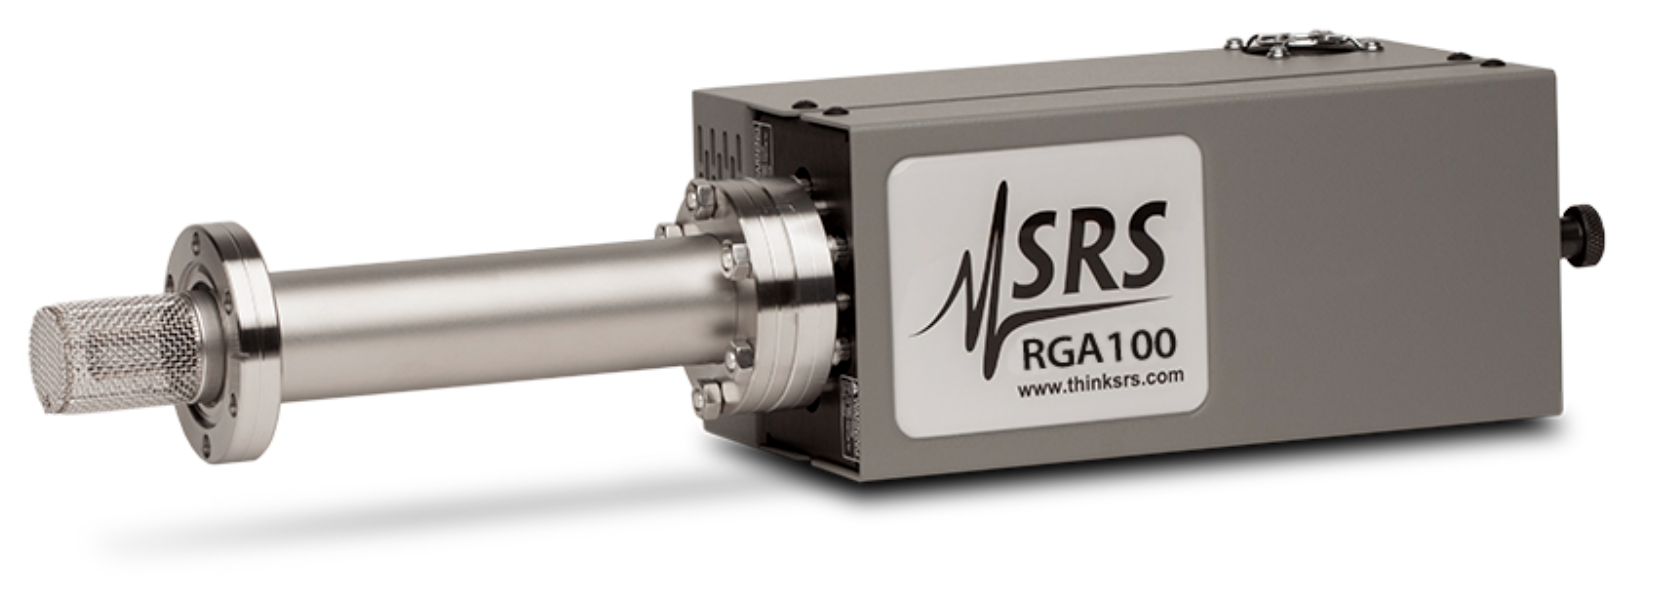
\includegraphics[width=0.6\linewidth]{figs/ch2-6.png}
	\caption{RGA100 残余气体分析仪实物图\cite{ResidualGasAnalyzer}}
	\label{fig:ch2-6}
\end{figure}

除实验过程中人为引入的高纯气体外，真空系统中还存在多种不可避免的残余气体来源。图\ref{fig:ch2-7}给出了在未通入外界气体条件下腔体内残余气体的组分分布。

\begin{figure}[htbp]
	\centering
	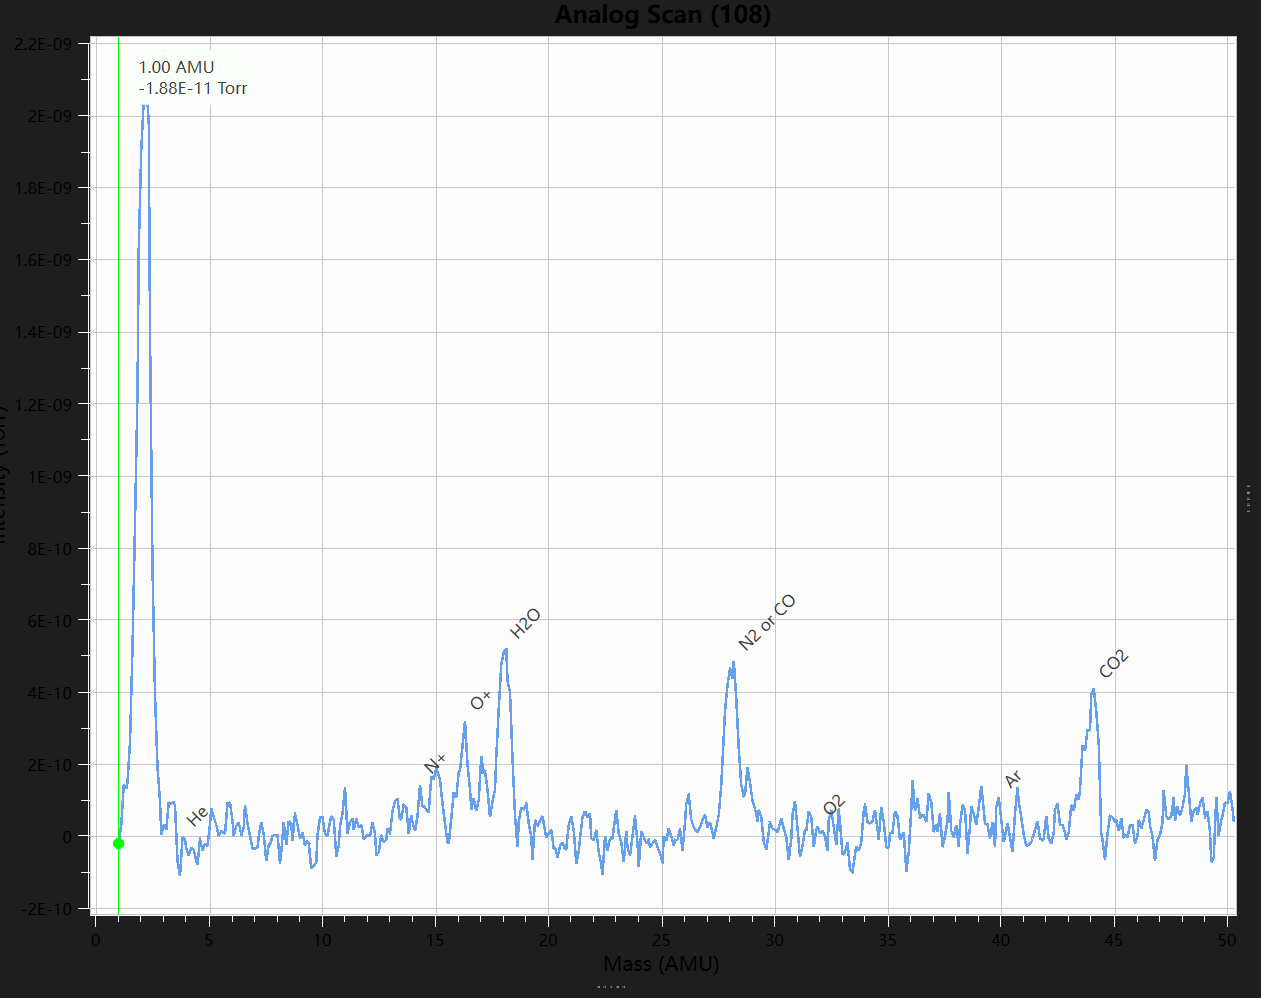
\includegraphics[width=0.6\linewidth]{figs/ch2-7.png}
	\caption{未通入外界气体时真空腔中残余气体的组分分布情况}
	\label{fig:ch2-7}
\end{figure}

首先，真空系统的泄漏是气体载入的重要来源之一。需要指出的是，“绝对无泄漏”的真空系统在实际中难以实现，工程上只能将泄漏控制在可忽略水平。常见泄漏位置包括 CF 法兰密封面、焊接接缝以及波纹管等结构薄弱区域。真实泄漏的一个典型特征是其残余气体组分比例与标准大气成分相近（例如 $\mathrm{N}_2$ 与 $\mathrm{O}_2$ 占主导）。然而，从图\ref{fig:ch2-7}可以看出，本系统中氢气占据主导地位，说明外界泄漏对气体本底的贡献较小，系统整体密封性能良好。

当系统经过充分抽气与烘烤处理后，材料本底出气成为限制极限真空度的主要因素。所谓材料出气，是指真空系统中结构材料及功能元件（如电离规灯丝、RGA 灯丝等）表面吸附或体相中溶解的气体，在真空环境下通过表面解吸或体扩散机制释放进入腔体的过程。本实验系统的主要材料包括不锈钢、玻璃以及无氧铜。在室温条件下，其主要出气组分为质量数为 $18~\mathrm{amu}$ 的水蒸气（$\mathrm{H}_2\mathrm{O}$）以及 $2~\mathrm{amu}$ 的氢气（$\mathrm{H}_2$）。

针对不同来源的气体，需要采用相应的烘烤除气策略。水蒸气主要来源于材料表面的物理吸附层，其去除依赖于中温烘烤（约 $150 \sim 200^\circ\mathrm{C}$），通过加速表面解吸过程可显著降低其分压；而氢气则主要来源于不锈钢材料体相中溶解的氢原子，其去除依赖于高温烘烤（通常 $\sim 300^\circ\mathrm{C}$），以促进氢在材料内部的扩散并逸出至真空环境中。经过长时间烘烤除气处理后，系统中水蒸气分压显著降低，而氢气逐渐成为超高真空环境中的主导气体组分，如图\ref{fig:ch2-7}所示。

最终，系统可稳定达到 $10^{-9}~\mathrm{Pa}$ 量级的超高真空水平，为冷原子体系的长寿命俘获及高精度真空计量提供必要条件。


\subsection{真空环境的维持与实时监测}

本实验中的超高真空环境由意大利 SAES Getters 公司研制的 NEXTorr\textsuperscript{\textregistered} Z200 一体化复合型超高真空泵维持。该装置将\textit{非蒸散型吸气剂（Non-Evaporable Getter, NEG）模块}与\textit{溅射离子泵（Sputter Ion Pump, SIP）模块}高度集成于标准全金属 ConFlat（CF）法兰结构中，实现了无油、无机械振动、无噪声的长期稳定运行，同时其内部无任何运动部件，具有极高的可靠性与运行寿命。

其中，NEG 模块采用 SAES 专利的 ZAO\textsuperscript{\textregistered}（Zr–V–Ti–Al）多孔烧结合金材料，能够通过化学吸附机制高效捕获活性气体分子。针对超高真空系统中占主导地位的氢气（\ce{H_2}），其峰值抽速可达 \SI{290}{\liter\per\second}，总吸气容量约为 \SI{1160}{torr\cdot\liter}。该泵的极限真空度优于 \SI{1e-11}{mbar}。此外，设备在结构设计上进行了低磁场优化，在距离泵体 \SI{10}{\centi\meter} 处的杂散磁场强度低于 \SI{1}{\micro\tesla}，从而有效避免对磁光阱（MOT）所需高均匀度磁场分布的扰动\cite{NEXTorrUHVPumps}。

NEG 与 SIP 模块的协同工作实现了对不同气体组分的互补抽气。具体而言，NEG 模块主要负责抽除活性气体（如 \ce{H_2}、\ce{CO}、\ce{N_2}、\ce{H_2O} 等），而 SIP 模块则用于抽除 NEG 难以有效捕获的惰性气体（如 He、Ar）。这种复合抽气机制能够在长时间尺度上稳定维持腔体内的超高真空环境，从而显著降低背景气体与冷原子的碰撞概率，延长原子俘获寿命，并提高冷原子真空计量的测量精度。

\begin{figure}[htbp]
	\centering
	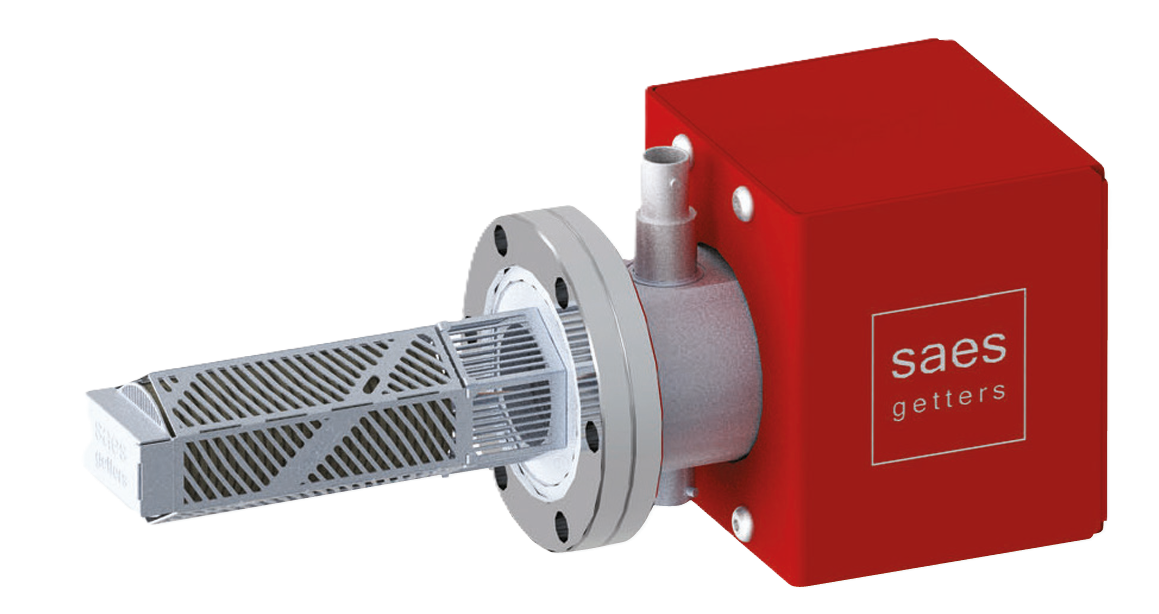
\includegraphics[width=0.6\linewidth]{figs/ch2-4.png}
	\caption{SAES Getters 公司生产的 NEXTorr\textsuperscript{\textregistered} Z200 一体化复合型超高真空泵\cite{NEXTorrUHVPumps}}
	\label{fig:ch2-4}
\end{figure}

在真空度的实时监测方面，本实验采用德国 Leybold 公司 COMBIVAC CM 52 真空控制器配合 IONIVAC IE 514 热阴极电离规，对主腔体压强进行连续测量。电离规基于气体分子在电子轰击下发生电离的原理，通过测量离子电流并结合其与气体数密度之间的近似线性关系，实现对真空压强的反演测量。该设备的测量范围覆盖 \(2 \times 10^{-12} \sim 1 \times 10^{-2}\ \text{mbar}\)，能够满足超高真空区间内高灵敏度与长时间稳定监测的需求\cite{COMBIVACCMPassive}。


\begin{figure}[htbp]
	\centering
	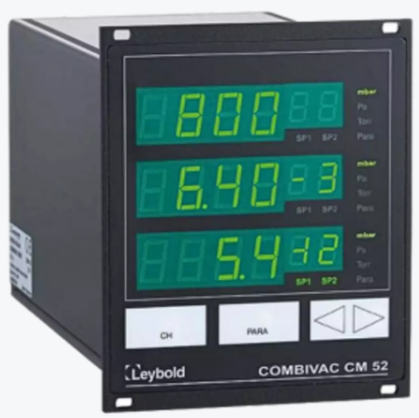
\includegraphics[width=0.3\linewidth]{figs/ch2-5.png}
	\caption{COMBIVAC CM 52 真空控制器\cite{COMBIVACCMPassive}}
	\label{fig:ch2-5}
\end{figure}

\section{激光系统}
\subsection{铷-87原子跃迁谱线}
激光冷却需要一个闭合的循环，但是很难保证准确的跃迁。加上一个泵浦光将暗态抽运回来，如图\ref{fig:ch2-11}。
\begin{figure}[htbp]
	\centering
	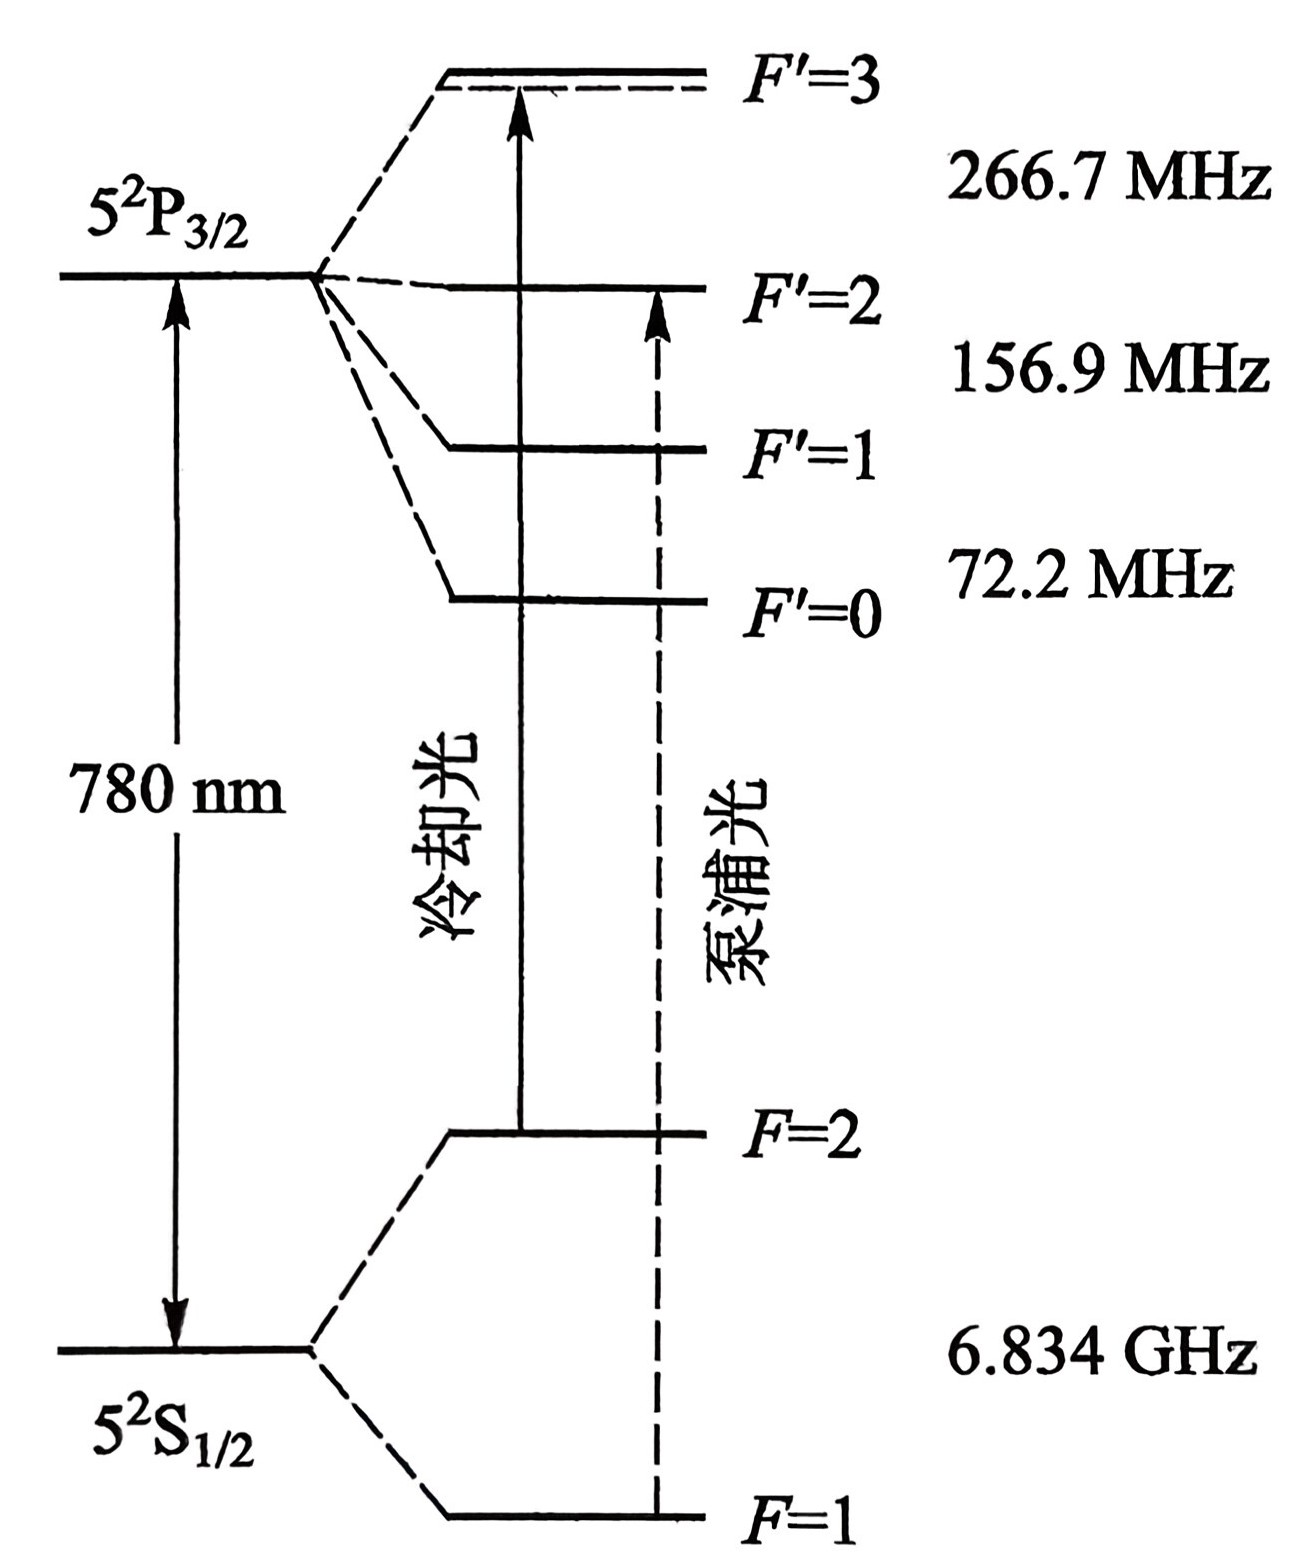
\includegraphics[width=0.4\linewidth]{figs/ch2-11.jpg}
	\caption{铷-87原子跃迁谱线}
	\label{fig:ch2-11}
\end{figure}
\subsection{光路设计}
\section{磁场系统}
\begin{figure}[htbp]
	\centering
	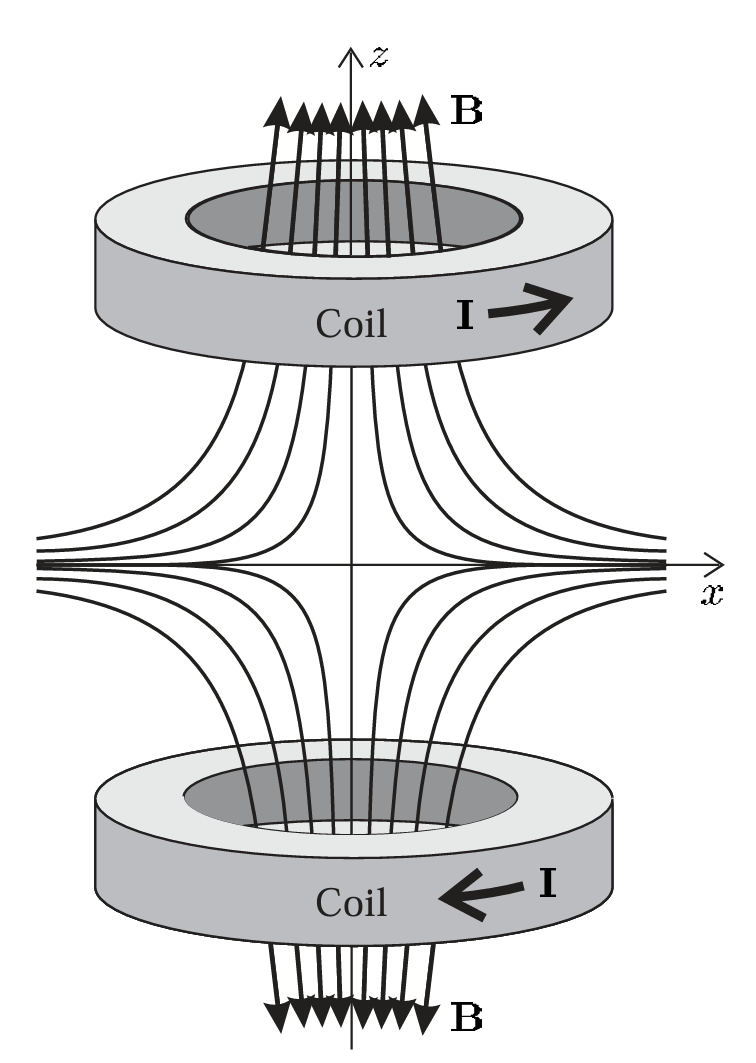
\includegraphics[width=0.4\linewidth]{figs/ch2-10.png}
	\caption{四极磁场}
	\label{fig:ch2-10}
\end{figure}
\begin{figure}[htbp]
	\centering
	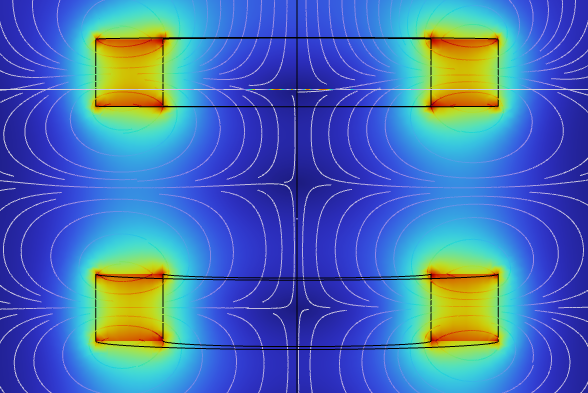
\includegraphics[width=0.5\linewidth]{figs/ch2-12.png}
	\caption{磁场模拟}
	\label{fig:ch2-12}
\end{figure}